\section{Auswertung}
\label{sec:Auswertung}
\subsection{Messdaten}
\label{sec:messdaten}
Die bei dem Versuch aufgenommenen Messdaten sind in den Tabellen \ref{tab:mess1} und \ref{tab:mess2}
dargestellt. 
%Wie zum Henker soll das passen??
\subsection{Das Emissionsspektrum der Kupfer Rontgenröhre}
\label{sec:emission}
Das nach Kaptiel \ref{sec:emissionsmessung} gemessene Emissionsspektrum wurde mittels \textit{matplotlib}\cite{matplotlib} 
als $\theta-N$ Diagramm in Abbildung \ref{fig:plot1} dargestellt. Dabei sind Bremsberg und die Spektrallinien $K_{\alpha}$ und 
$K_{\beta}$ des Kupfers makiert. Die Punkte der jeweiligen Extrema sind in Tabelle \ref{tab:hp} dargestellt und in Abbildung 
\ref{fig:plot1} rot unterlegt. Bei $K_{\alpha}$ und $K_{\beta}$ sind zudem noch die charakteristischen Spektrallinien des Kupfers
eingezeichnet. 
\begin{table}[H]
    \centering
        \caption{Extrema des Emissionsspektrums}
        \label{tab:hp}
        \sisetup{table-format=4.1}
        \begin{tabular}{S S S}
          \toprule
          {Extremum} & {$\theta [°]$} & {$N [\si{\per\second}]$} \\
          \midrule
          {Bremsberg }   & 11.1 & 420.0 \\
          {$K_{\beta} $} & 20.2 & 1599.0\\
          {$K_{\alpha}$} & 22.5 & 5050.0\\
          \bottomrule
        \end{tabular}
      \end{table}

\begin{figure}[H]
    \centering
    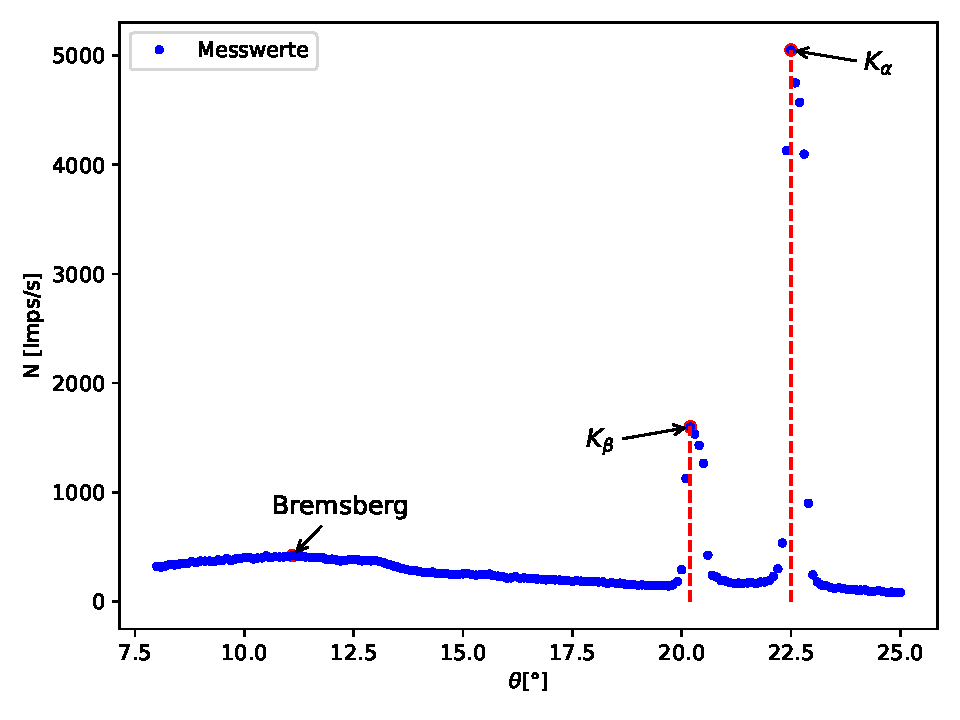
\includegraphics[scale = 0.9]{auswertung/plot1.pdf}
    \caption{$\theta-N$ Darstellung des Emissionsspektrums.}
    \label{fig:plot1}
\end{figure}
\noindent
Für die Spektrallinien wird nun die Wellenlänge $\lambda$ mittels Gleichung \eqref{eqn:(3)} berechnet und mit dem Zusammenhang
\eqref{eqn:E=hc/lambda} als Energie angegeben. Die Ergebnisse finden sich in Tabelle \ref{tab:energie}.
\begin{table}[H]
    \centering
        \caption{Photonenergie bei $K_{\alpha}$ und $K_{\beta}$}
        \label{tab:energie}
        \sisetup{table-format=4.1}
        \begin{tabular}{S S S S}
          \toprule
          {Spektrallinie} & {Energie $[\si{\kilo\electronvolt}]$} & {Literaturwert \cite{AP03} $[\si{\kilo\electronvolt}]$} & {Abweichung [\%]}\\
          \midrule
          {$K_{\alpha}$} & 8.044 & 8.048 & 0.0472 \\
          {$K_{\beta} $} & 8.915 & 8.907 & -0.091 \\
          \bottomrule
        \end{tabular}
      \end{table}

\subsection{Bestimmung der Transmission als Funktion der Wellenlänge}
\label{sec:transmission}
Um die Transmission $T$ zu errechnen werden nach Gleichung \eqref{eqn:trans} $I_{0}$ und $I_{Al}$ benötigt. Diese werden aus den Messdaten
aus Tabelle \ref{tab:mess2} mittels Gleichung \eqref{eqn:(4)} berechnet. Die so gewonnene Transmission wurde dann mittels 
\textit{matplotlib} \cite{matplotlib} in einem $\lambda-T$ Diagramm in Abbildung \ref{fig:plot2} aufgetragen. Dabei ist die Wellenlänge
$lambda$ zuvor wieder mit mittels Gleichung \eqref{eqn:(3)} berechnet worden. Die angegebenen Fehlerbalken beruhen auf der Poisson-Verteilung
$\Delta N=\sqrt{N}$.
\begin{figure}[H]
    \centering
    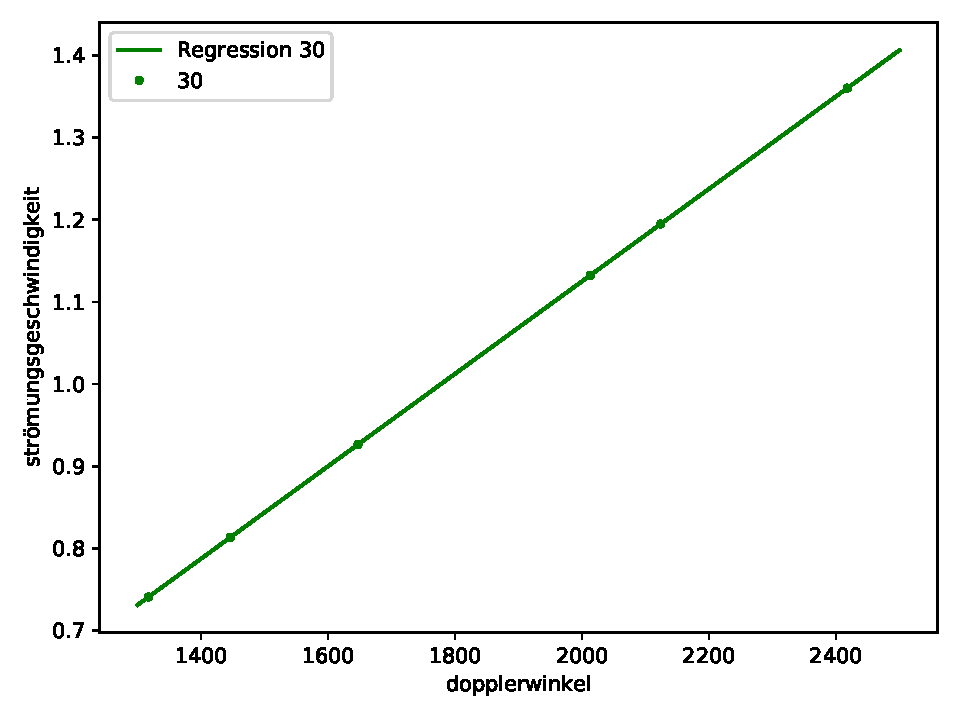
\includegraphics[scale = 0.9]{auswertung/plot2.pdf}
    \caption{Die Transmission in Abhängingkeit der Wellenlänge.}
    \label{fig:plot1}
\end{figure}
\noindent
Die eingezeichnete Regression hat dabei eine Funktionsgleichung der Form
  \begin{equation*}
      y=a\cdot x+b \label{eqn:gerade}
  \end{equation*} 
mit
  \begin{align*}
    a &= \SI{-0.015 \pm 0.000}{\per\pico\metre}\\
    b &= \SI{1.225 \pm 0.014}.
  \end{align*}
Die Unsicherheiten wurden dabei von  \textit{numpy} \cite{numpy} berechnet.

\subsection{Bestimmung der Compton-Wellenlänge}
\label{sec:compton}
Für die Bestimmung der Compton-Wellenlänge $\lambda_c$ werden nach \ref{sec:diskussion3} $I_0$, $I_1$ und $I_2$ benötigt.
Die Messung ergab
\begin{align*}
    I_0 &= 2731 \si{Imp}\\
    I_1 &= 1180 \si{Imp}\\
    I_2 &= 1024 \si{Imp}.
\end{align*}  
Durch diese werden die Transmissionen $T_1=I_1/I_0$ und  $T_2=I_2/I_0$ berechnet, womit sich dann die Wellenlänge durch Gleichung
\eqref{eqn:lambda} berechnen lässt. Dafür werden die Parameter der linearen Regression verwendet, also wird \eqref{eqn:lambda} zu
\begin{equation*}
    \lambda_i = \frac{T_i -b}{a}. 
\end{equation*}
Einsetzen der berechneten Werte ergibt dann
\begin{align*}
    \lambda_1 &= \SI{52.189}{\pico\metre}\\
    \lambda_2 &= \SI{55.948}{\pico\metre}.
\end{align*}
Somit ist die berechnete Compton-Wellenlänge
\begin{equation*}
    \lambda_c=\lambda_2-\lambda_1= \SI{3.7593}{\pico\metre}.
\end{equation*}